% Einstellung der Dokumentklasse für A4 und weitere Optionen
\documentclass[a4paper, 12pt, bibliography=totoc, listof=totoc, parskip=half, numbers=noenddot, oneside]{scrreprt} % ONESIDE
%\documentclass[a4paper, 12pt, bibliography=totoc, listof=totoc, parskip=half, numbers=noenddot, twoside]{scrreprt} % TWOSIDE

% Mathematische Zeichen in der Überschrift werden ebenfalls fett gesetzt
\addtokomafont{disposition}{\boldmath} 

% scrhack ersetzt in den Packages hyperref, float und listings einige Makros für bessere KOMAScript-Kompatibilität (muss vor den betreffenden Packages aufgerufen werden)
\usepackage[]{scrhack}

% Deutsch nach neuer Rechtschreibung
\usepackage[english, ngerman]{babel}

% Automatische Ersetzung der Umlaute
\usepackage[utf8]{inputenc}

% Erweiterter Zeichensatz incl. Umlaute
\usepackage[T1]{fontenc}

%% Times als Schriftart
%\usepackage{mathptmx}
%\usepackage[scaled=.95]{helvet} 
%\usepackage{courier}

%% Latin Modern als Schriftart
%\usepackage{lmodern}

%% Arial bzw. Helvetica als Schriftart (excl. Formelsatz)
%\renewcommand{\familydefault}{\sfdefault}
%\usepackage{helvet}



% Palatino als Schriftart
\usepackage{mathpazo}
\usepackage[scaled=.95]{helvet}
\usepackage{courier}

% Kopf- und Fußzeilen
\usepackage[automark, headsepline]{scrpage2}

% Kopf- und Fußzeile definieren
\pagestyle{scrheadings}
\renewcommand{\headfont}{\bfseries}
\clearscrheadfoot
\ohead{\headmark}                              
\cfoot{\pagemark} % ONESIDE
%\ofoot{\pagemark} % TWOSIDE

% Einstellung der Seitenränder
\usepackage[includeheadfoot]{geometry}

%Seitenränder für A4
\geometry{includeheadfoot, headsep=1.9cm, left=2.9cm, right=2.4cm, top=1.6cm, bottom=1.25cm, footskip=1.3cm, footnotesep=1cm}

% Einstellen der Schriftgröße der Bildbeschriftungen
\setkomafont{captionlabel}{\itshape}
\setkomafont{caption}{\itshape}

% Einstellen der Schriftarten der Überschriften
\setkomafont{chapter}{\Large}
\setkomafont{section}{\large}
\setkomafont{subsection}{\large}

%Umbruch in Formeln
 \usepackage{eqnarray}
 
 %Zellen farblich hervorheben in Tabellen
 \usepackage{colortbl}


% Abstand zwischen Bild und Beschriftung
\setlength{\abovecaptionskip}{7pt}

% Anpassen der Trennungs-/Umbruchparameter zum Verhindern von "overfull \hbox"
\setlength\emergencystretch{3em}
\tolerance=1000

% Gliederungstiefe festlegen
\setcounter{secnumdepth}{3} 
\setcounter{tocdepth}{3} 

% Formatierung von Inhalts- und Abbildungsverzeichnis
\usepackage[titles]{tocloft}

\cftsetpnumwidth{1.0cm}

\setlength\cftchapnumwidth{0.8cm}
\setlength\cftsecnumwidth{1.2cm}
\setlength\cftsubsecnumwidth{1.5cm}
\setlength\cftsubsubsecnumwidth{1.8cm}
\setlength\cftfignumwidth{1.4cm}

\setlength\cftchapindent{0cm}
\setlength\cftsecindent{0.8cm}
\setlength\cftsubsecindent{2.0cm}
\setlength\cftsubsubsecindent{3.5cm}

\renewcommand{\cftchapaftersnum}{}
\renewcommand{\cftsecaftersnum}{}
\renewcommand{\cftsubsecaftersnum}{}
\renewcommand{\cftsubsubsecaftersnum}{}
\renewcommand{\cftfigaftersnum}{}

% Optischer Randausgleich 
\usepackage{microtype}

% Einbinden von Grafiken
\usepackage{graphicx}

% Silbentrennung in Überschriften
\usepackage{ragged2e}
\renewcommand*{\raggedsection}{\RaggedRight}     

% Grafiken mit [H] als Parameter zwingend an der Aufrufstelle platzieren
\usepackage{float}

% E-TeX aktivieren, um mehr \dimens freizugeben
%\usepackage{etex}

% Ermöglicht segmentierte Matrizen
\usepackage{easymat}

% Formelsatz in fett
\usepackage{bm}

%\usepackage{floatrow}

% Verhindert Einbinden von Grafiken vor ihrer Aufrufstelle
\usepackage{flafter}

% Mehrere Grafiken nebeneinander
\usepackage{subcaption}


% Schönerer Formelsatz
\usepackage{amsmath, amssymb}
% Komma als Dezimaltrennzeichen interpretieren
\usepackage{icomma}

% Zeichen für math. Transformationen
\usepackage{trfsigns}

% setspace für Längeneinstellungen mit \setlength usw.
\usepackage{setspace}

% Tabellensatz
\usepackage{booktabs}
\usepackage{array}
\usepackage{tabularx}
\usepackage{Tabbing}
\usepackage{longtable}
\usepackage{ltablex}
\usepackage{dcolumn} % Tabellenzeilen am Dezimalpunkt ausrichten

\newcolumntype{L}[1]{>{\raggedright\arraybackslash}p{#1}} % linksbündig mit Breitenangabe
\newcolumntype{C}[1]{>{\centering\arraybackslash}p{#1}}   % zentriert mit Breitenangabe
\newcolumntype{R}[1]{>{\raggedleft\arraybackslash}p{#1}}  % rechtsbündig mit Breitenangabe

% Listen/Aufzählungen mit Tabulatoren
\usepackage{listliketab}
\usepackage{paralist}

% make enum items configurable
\usepackage{enumitem}

% Breite horizontale Linie mit \whline (benötigt booktabs)
\newcommand\whline{\specialrule{1.5pt}{0pt}{0pt}}


% Sonderzeichen und griechische Buchstaben im normalen Text
\usepackage{textcomp}

% Euro-Zeichen €
\usepackage{eurosym}

% Zahlen mit Einheiten setzen
\usepackage{siunitx}
% \usepackage{unitsdef}

% Farbe im Dokument
\usepackage{xcolor} 

% Nummerierung von Nicht-Gleitobjekten
% \usepackage{nonfloat, capt-of}

% Formatierten Quellcode einbinden
% \usepackage{listings, keyval}

% Dirty Trick, um align-Umgebung in amsmath abkürzen zu können
% (das obsolete eqnarray funktioniert aber mit newcommand)
\def\beqar#1\eeqar{\begin{align*}#1\end{align*}}
\def\beqarn#1\eeqarn{\begin{align}#1\end{align}}

% Strafpunkte für Schusterjungen und Hurenkinder
\clubpenalty = 1000
\widowpenalty = 1000 
\displaywidowpenalty = 1000

% Grafiken werden erst ab 75% Seitenhöhe alleine auf eine float page gesetzt
\renewcommand{\floatpagefraction}{0.75}

% Floatobjekte, die alleine auf einer Seite stehen, werden nach oben statt vertikal zentriert gesetzt
\makeatletter
\setlength{\@fptop}{0pt}
\makeatother

% Theorem-Umgebung
\usepackage{amsthm}
% \newtheorem{Name der Umgebung}{Angezeigter Ausdruck}
\newtheorem{Erkenntnis}{Erkenntnis}

% Zitieren im Autor-Jahr-Schema
\usepackage[numbers]{natbib}


%Weitere Optionen für natdin_iwb.bst:
\makeatletter
\newcommand{\bibstyle@natdin}{%

%Formatierung der Literaturverweise im Fließtext
\bibpunct{(}{)}{;}{a}{}{,~}

%Literaturverzeichnis: Labels fett / Zeilenumbruch nach Labels
\gdef\NAT@biblabelnum##1{\textsc{\textbf{##1}}\\}} %

\bibstyle@natdin

% Einzug der Belege nach dem Label im Literaturverzeichnis
\setlength{\bibhang}{7mm} 

\makeatother


% Kein Seitenumbruch von Fußnoten
\interfootnotelinepenalty=10000

% Rahmen mit \begin{frame} ... \end{frame}
% \usepackage{framed}

% Benutzung von Hintergründen
%\usepackage{everyshi}
%\usepackage{eso-pic}
%\usepackage{calc}
%\usepackage{ifthen}
%\usepackage{wallpaper}

% Anführungszeichen mit \enquote
\usepackage[autostyle,german=guillemets]{csquotes}

% Einbindung von PDF
\usepackage{pdfpages}

% landscape
\usepackage{pdflscape}

% Verfasser und Betreuer ausrichten
\usepackage[absolute]{textpos}

%Tabellen- und Abbildungsnummerierung ohne Kapitelnummer
\usepackage{chngcntr}
\counterwithout{figure}{section}
\counterwithout{table}{section} 
\counterwithout{equation}{section}
\counterwithin{figure}{chapter}
\counterwithin{table}{chapter} 
\counterwithin{equation}{chapter}


% Definition eigener Befehle/Abkürzungen
\newcommand{\beq}{\begin{equation*}}
\newcommand{\eeq}{\end{equation*}}
\newcommand{\beqn}{\begin{equation}}
\newcommand{\eeqn}{\end{equation}}
\newcommand{\bssp}{\begin{spacing}{1}}
\newcommand{\essp}{\end{spacing}}
\newcommand{\nl}{\\[0,3cm]}
\newcommand{\entspricht}{\mathrel{\widehat{=}}} 
\newcommand{\diag}{\mathrm{diag}}
\newcommand{\res}{\mathrm{res}}
\newcommand{\ges}{\mathrm{ges}}
\newcommand{\reduce}{\mathrm{red}}
\newcommand{\tats}{\mathrm{tats}}
\newcommand{\soll}{\mathrm{soll}}
\newcommand{\abw}{\mathrm{abw}}
\newcommand{\ber}{\mathrm{ber}}
\newcommand{\Steuer}{\mathrm{Steuer}}
\newcommand{\Aktor}{\mathrm{Aktor}}
\newcommand{\Sensor}{\mathrm{Sensor}}
\newcommand{\Eck}{\mathrm{Eck}}
\newcommand{\Feder}{\mathrm{Feder}}
\newcommand{\krit}{\mathrm{krit}}
\newcommand{\theo}{\mathrm{theo}}
\newcommand{\real}{\mathrm{real}}
\newcommand{\Verst}{\textrm{Verstärker}}
\newcommand{\grad}{\ensuremath{^\circ}}
\newcommand{\iwb}{\textit{iwb} }


%Alle Abkürzungen müssen im Abkürzungsverzeichnis erklärt werden!
\newcommand{\zb}{z.\,B.}
\newcommand{\og}{o.\,g.}
\newcommand{\ua}{u.\,a.}
\newcommand{\ie}{d.\,h.}
\newcommand{\Dh}{D.\,h.}
\newcommand{\zt}{z.\,T.}
\newcommand{\zz}{z.\,Z.}
\newcommand{\idr}{i.\,d.\,R.}

%1,5-facher Zeilenabstand
\onehalfspacing

% Links im pdf-Dokument setzen (sollte ganz am Ende geladen werden!)
\usepackage{hyperref}

% Units verwenden
\usepackage{units}

\usepackage[miktex]{gnuplottex}

% \def\acrobat{\hyperdef{jump}{here}{}}
%Semi-automatic forward search
%An much more useful solution would be to use the hyperref package:
%
%1. Make sure the hyperref package is loaded: \usepackage{hyperref}
%
%2. Define the following command: \def\acrobat{\hyperdef{jump}{here}{}}
%
%3. Change the "view project's output" and "forward search" DDE command (as described earlier on) to: command: [DocOpen("%bm.pdf")][FileOpen("%bm.pdf")][DocGoToNameDest("%bm.pdf","jump.here")]
%
%4. Use somewhere in the text (usually, where you are currently working…) the new command \acrobat and, after (re)opening, the reader should jump to that location.
%
%Note that steps 1. and 2. have to be done in the header of your document. If you use pdfTeX, you should load the hyperref package via \usepackage[pdftex]{hyperref}; if you use dvips, load it using \usepackage[dvips]{hyperref}. If several \acrobat commands are issued, the reader always jumps to the "latest" one.

%% URLs umbrechen (nach hyperref aufrufen!)
%\usepackage{breakurl}

% closing roots http://tex.stackexchange.com/questions/29834/closed-square-root-symbol#answer-29838
\usepackage{letltxmacro}
\makeatletter
\let\oldr@@t\r@@t
\def\r@@t#1#2{%
\setbox0=\hbox{$\oldr@@t#1{#2\,}$}\dimen0=\ht0
\advance\dimen0-0.2\ht0
\setbox2=\hbox{\vrule height\ht0 depth -\dimen0}%
{\box0\lower0.4pt\box2}}
\LetLtxMacro{\oldsqrt}{\sqrt}
\renewcommand*{\sqrt}[2][\ ]{\oldsqrt[#1]{#2}}
\makeatother


\usepackage{epstopdf}

% http://ctan.org/pkg/adjustbox
\usepackage[export]{adjustbox}

% Listings
\definecolor{lst_comment}{HTML}{008000}
\definecolor{lst_string}{HTML}{A31515}
\definecolor{lst_numbers}{HTML}{2B91AF}

\usepackage{listings}
\lstset{language = C++}

 \lstset{
   basicstyle=\scriptsize\ttfamily\scriptsize,
   keywordstyle=\bfseries\ttfamily\color{blue},
   stringstyle=\color{lst_string}\ttfamily,
   commentstyle=\color{lst_comment}\ttfamily,
	 %identifierstyle=\color{blue},
   emph={square}, 
   emphstyle=\color{blue}\texttt,
   emph={[2]root,base},
   emphstyle={[2]\color{yac}\texttt},
   showstringspaces=true,
   flexiblecolumns=false,
   tabsize=4,
   numbers=left,
   numberstyle=\tiny\ttfamily\bfseries\color{lst_numbers},
   numberblanklines=false,
   stepnumber=1,
   numbersep=6pt,
   xleftmargin=17pt,
	 breaklines = true,
 }

% Weist pdflatex an, die Ausgabe in pdf-Version 1.6 vorzunehmen.
% Das vermeidet Fehler mit eingebundenen pdfs > v1.4
\pdfminorversion=6


\hypersetup{
	pdfauthor={Vorname Nachname},
	pdftitle={Titel der Arbeit},
	pdfsubject={Studienarbeit an der TU München, Lehrstuhl MiMed, Garching},
	pdfkeywords={{TUM}},
	pdfborder={0 0 0},
	pdfcreator={LaTeX}
}

%
\numberwithin{figure}{section}
\numberwithin{table}{section}
\numberwithin{equation}{section}
\AtBeginDocument{\numberwithin{lstlisting}{section}}

% take text in circles little bit lower to make it better looking

\let\textcircledold\textcircled
\let\textcircled\relax
%\newcommand{\textcircled}[1]{\raisebox{.5pt}{\textcircledold{\raisebox{-.9pt} {#1}}}}

\usepackage{tikz}
\newcommand*\textcircled[1]{\tikz[baseline=(char.base)]{
    \node[shape=circle,draw,inner sep=2pt] (char) {#1};}}

\usepackage{multicol}

% Check if all labels are referenced
%\usepackage{refcheck}

%eigene Farben
\definecolor{drot}{rgb}{0.5,0,0} 
\definecolor{dgruen}{rgb}{0,0.5,0} 
\definecolor{dblau}{rgb}{0,0,0.5}
\definecolor{lila}{rgb}{0.5,0,0.5} 
\definecolor{rosa}{rgb}{1,0,1} 
\definecolor{dgelb}{rgb}{0.5,0.5,0} 
\definecolor{turkis}{rgb}{0,1,1} 

%fuer Matlab-Quellcode-Darstellung
\usepackage[numbered,framed]{mcode}




\begin{document}
\renewcommand{\figurename}{Figure}
\renewcommand{\contentsname}{Table of Contents}
\renewcommand{\bibname}{Bibliography}
\renewcommand{\listfigurename}{Figure List}
	
\pagenumbering{Roman}

\thispagestyle{plain}


\begin{textblock*}{9 cm}(27mm,15mm)

\includegraphics[valign=t]{grafiken/MW_CMYK.eps}
\hspace{5 mm}

\includegraphics[valign=t]{grafiken/MED_CMYK.eps}
\hspace{5 mm}

\includegraphics[valign=t]{grafiken/MiMed.eps}
\end{textblock*}

\begin{textblock*}{2 cm}(17.7 cm, 15mm)

\includegraphics[]{grafiken/TUMLogo_oZ_Outline_blau_CMYK.eps}
\end{textblock*}

\hspace{5 mm}

\begin{center}
\begin{singlespace}
\small Technical University of Munich\smallskip\\
Department of Mechanical Engineering\smallskip\\
Institute of Micro Technology and Medical Device Technology\smallskip\\
Univ.-Prof. Dr. Tim C. Lüth
\end{singlespace}
\end{center}
\vspace{0.8 cm}
\begin{center}
{\large Master's Thesis}
\end{center}
\vspace{0.70 cm}
\begin{center}
{\Large Investigation of the Coloring Behavior of Zirconiumdioxide ($ZrO_2$) Dental Ceramics by Ink-jet Printing of Metal-ionic Inks}
\end{center}
\vspace{0.70 cm}
\begin{center}
{\large Furkan Öztürk\nl
Matr.-Nr.: 03668338}
\end{center}

%% Betreuer einfügen
\begin{textblock*}{80 mm}(27mm,21cm)%
\begin{singlespace}
\begin{tabular}{p{3.5cm}p{7cm}}

Supervising \mbox{University Prof.
}:  & \hspace{20cm} \mbox{} Univ.-Prof. Dr. Tim C. Lüth \nl
\end{tabular}
\end{singlespace}
\begin{tabular}{p{3.5cm}p{7cm}}
Supervisor: & Dipl.-Ing. Dominik Rumschöttel \nl

Issued on: & 01.10.2017 \nl

Submitted on: & 29.03.2018 \nl
\end{tabular}
\end{textblock*}

\cleardoublepage
%%%%%%%%%%%%%%%%%%%%%%%%%%%%%%%%%%%%%
\addchap{Ehrenwörtliche Erklärung}%
%%%%%%%%%%%%%%%%%%%%%%%%%%%%%%%%%%%%%

Ich erkläre hiermit ehrenwörtlich, dass ich die vorliegende Arbeit selbstständig und ohne Benutzung anderer als der angegebenen Hilfsmittel angefertigt habe; die aus fremden Quellen (einschließlich elektronischer Quellen) direkt oder indirekt übernommenen Gedanken sind ausnahmslos als solche kenntlich gemacht.
% Die Arbeit wurde bisher keiner anderen Prüfungsbehörde vorgelegt.
\vspace{1cm}\\
Garching bei München, den 29.03.2018
\vspace{2.5cm}\\
Furkan Öztürk

\cleardoublepage
\addchap{Foreword}

Diese Arbeit entstand am....

An dieser Stelle möchte ich...

Ebenso danke ich ....

\vfill
Garching bei München, March 2018

Furkan Öztürk

% \include{aufgabenstellung}

% Automatische Kolumnentitel
\automark{chapter} % ONESIDE
%\automark[section]{chapter} % TWOSIDE

\cleardoublepage
\tableofcontents
%\chapter*{Inhaltsverzeichnis}
%\addcontentsline{toc}{chapter}{Inhaltsverzeichnis}

\cleardoublepage
\pagenumbering{arabic}

\cleardoublepage
\counterwithout{figure}{section}
\counterwithout{table}{section} 
\counterwithout{equation}{section}
\counterwithin{figure}{chapter}
\counterwithin{table}{chapter} 
\counterwithin{equation}{chapter}


\chapter{Introduction}
\label{sec:problemstellung}
 Only in Germany more than 1 Million teeth are replaced annually. The replacement procedure is accomplished with an implantation of the tooth replica to provide the aesthetics and the function of the natural tooth. Ancient Egyptians used tooth shaped ivory to regain the function of the missing teeth. Today the technology has evolved to a point where the dental replacement for a single tooth is an assembly of three parts, which  are to be seen in Figure 1.1. The implant is the part which is screwed to the lower jaw bone (mandible) and anchors the whole replacement assembly to the chin. The preferred material used for the implant are titanium in the EU and tantalum in the US. The enhanced osseointegration of the porous implant material surface, biocompatibility of the ceramic interface, formed due to the surface oxidation a Young's Modulus, which is similar to the human bone are the main reasons for titanium and tantalum to be the prime materials for this purpose. The abutment takes on the task of a fitting  for the crown and is made of the same material as the implant.
  \begin{figure}[h]
 	\centering
 	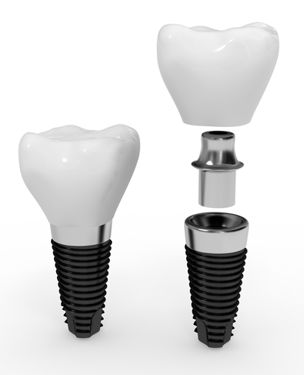
\includegraphics[width=0.4\textwidth]{grafiken/implant.png}
 	\caption{Single tooth replacement}
 	\label{fig:implant}
 \end{figure} 
 
 The crown of the tooth replacement is the part which imitates the visual qualities of the tooth. There are several material, which a crown can be made of or assembled from. The most popular crown material dominating the market is the Yttria-stabilized zirconia (YSZ), which has a cubic fluorite crystal structure and is going to be referred as zirconia in the frame of this thesis. However, zirconia in its pure form is a plain white material with high translucency. In case of single tooth replacement  the newle implanted crown would be absurdly white when compared to the neighboring teeth.Even when a full chin dental replacement is conducted, it is abnormal to have a full set of plain white teeth without any shading. This situation makes it a necessity to preprocess the crowns to match the neighboring teeth or another natural shade of choice in case of a fully monolithic replacement. Dentist are using a shade guide seen in the figure \ref{fig:shadeguide} for a side-by-side comparison to determine the color and the shade of the teeth. One can observe that there are 4 color groups A, B, C and D which are referred as orange-brown, yellow, grey-brown and red respectively \citep{vita}. Each of these colors have shades ranging from 1 to 4. Even though the shades are coded with the numbers from 1 to 4 with increments of 0.5 a total analogue shade acquisition is possible. The number 1 represents the shade with the least and 4 with the most saturated tone for each color.
 \newline
 \begin{figure}[h]
 	\centering
 	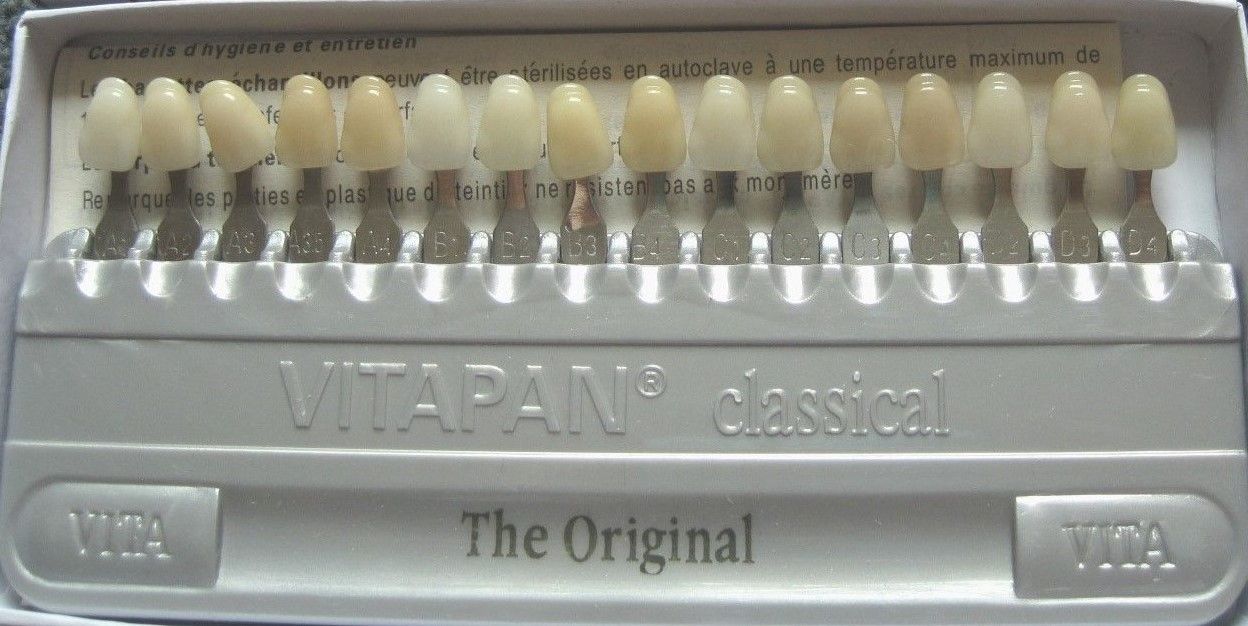
\includegraphics[width=0.9\textwidth]{grafiken/shadeguide.jpg}
 	\caption{Vitapan Shadeguide}
 	\label{fig:shadeguide}
 \end{figure}  
 


\chapter{State of the Research}
\label{sec:stand_forschung}

Addressing the shading process of the dental zirconia-based ceramics as a combined procedure of drop generation, dispersion of the ink within the porous material and post sinter generation of the color below the surface of the porous material, it can be said that the quantitative coloring process of the dental crowns is an uncharted area for the scientific researches in the present-day. There have been some research made in the fields concerning the absorption of the liquid by materials presenting a porous inner structure and permeable surface conditions. How the liquid is distributed inside the material, what are the effects of the pore sizes, forms and distributions is investigated by various teams from all around the world for a variety of liquids and porous materials. 



\section{Structure of the Porous Medium}

The crystallographic state of zirconia depends on the temperature under atmospheric pressure. Until reaching a temperature of {1170\textdegree} Celcius the crystallographic structure shows a monoclinic symmetry. After that temperature the structure can be defined as tetragonal until {2370\textdegree} C , which afterwards becomes cubic up to the melting point. The volume of the material increases about 4.5\% during the transformation from tetragonal to monoclinic phases, which is enough to cause a crack induced failure. This evitable transformation begins at about {950\textdegree} C while cooling down and the only way to stabilize the tetragonal structure is creating CaO, MgO, $Y_{2}O_{3}$ or $CeO_{2}$ oxides inside the structure to keep the tetragonal formation  at room temperature, which eliminates the crack induction and therefore the structural failure of the material parallel to an enhanced toughness. \citep{denry2008state}

On a different aspect, some research has been conducted about the effect of the coloring process on the structural strength of the zirconia. In the research of Shah et al. coloring zirconia with cerium acetate mixtures with a maximum ink weight ratio of 5\% provided a distinctive shade and did not cause a mechanical disadvantage. However, the ratios above 5\% have decreased the mechanical properties while not increasing the shading level significantly. The paper also includes data for case where the coloring process is conducted using cerium chloride and bismuth chloride. For both cases 1\% coloring agent was the limit, if the flexural strength was to be conserved. The low temperature degradation was also observed in the frame of the paper, which did not show any co-dependence with the coloring solution.\citep{shah2008effect}

\section{Ink Distribution and Infiltration Time}
In 2016 Lee et al. have investigated the absorption behavior of water drops impinging porous stones experimentally and numerically. The investigation includes the phases from spreading to evaporation for a water droplet considering the absorbed amount of the droplet during the depletion and spreading of the humidity within the manner depending on time for three porous materials. Quantitative measurements of the water absorption for the materials are conducted with high-speed imaging and neutron radiography methods during the time range from the impact moment to the end of the spreading phase after absorption. Neutron radiography shows a high resolution quantitative distribution of absorbed water. During the first contact and deposition on the surface the droplets do not exhibit a wetting behavior.  As soon as the droplet acquires its maximum diameter on the surface, it gets fixed and the contact angle with the surface remains constant as long as the droplet is not drained by the stone. The absorption behavior doesn’t have the same attributes throughout the whole process. At the beginning the material shows a contact resistance blocking the absorption, which is associated with the entrapped air beneath the area encapsulated by the borders of the water droplet. In the second phase the encapsulated air finds a way to diffuse away so the capillary flow takes place flawlessly until the total disappearance of the droplet on the surface is observed. The experimental data shows accordance to the phases of the numerical model for water flow inside the unsaturated porous material. The collision velocity has a huge effect on drop spreading on the surface and impregnation, but not so much on the distribution of the water after the initial absorption. The absorption and distribution rates are highly relevant to the capillary structure of the stones.\citep{lee2016absorption}


Pecho et al. have conducted experiments to analyse the optical behaviour of dental zirconia and dentin in comparison utilizing Kubelka-Munk theory. The results show that the current zirconia materials alone could not satisfy the luminous transmittance of the natural dentin so an additive application of masking is required to reach an approximate to the natural tooth.\citep{pecho2015optical}

The infiltration time of the porous medium was formulated by Markicevic et al. in 2009 as:

\begin{equation}\label{eq:InfTime}
t_{in}=\kappa \cdotp {\frac{\mu \cdotp r{_0}^{1.85}}{\sigma \cos({\theta})\varPhi^{0.38}}}
\end{equation}
\newline
$t_{in}$ defines the infiltration time and depends on the parameters $\kappa$ , which is the permeability constant of the medium and $\mu$ the kinematic viscosity of the fluid. The initial drop radius is symbolized by $r_{0}$. $\theta$ stands for the initial contact angle after the impact of the droplet on the surface. The $\sigma$ in the denominator is the surface tension of the liquid. The higher the surface tension is the harder it is for the liquid to wet the surface of the material because of the increased contact angle and hardened impregnation capability. The last dependency of the infiltration time is  the $\phi$ constant for the material, identifying the porosity level of the material. \citep{markicevic2009infiltration}

Stratov et al. have provided experimental results regarding  the spreading phases of silicon oil droplets utilizing capillary forces over different permeable layers and observing the diameters of the droplets and wetted areas over time. They have divided the depletion into two phases, of which the first one is defined by the time to reach the maximum diameter for the drop base and the second one is identified by the reduction of the drop base while the depletion takes place. The findings of the experiments show that the different oils on the different porous material with similar porosity and mean pore dimensions. showed similar spreading characteristics on a different time scale and the contact angle remained constant throughout the second stage.\citep{starov2002thick}

The dispersion behavior of liquid drops inside porous media which are previously saturated with the identical liquid are examined in the work of Starov et al. The study was conducted considering both theoretical and experimental perspectives. The study was conducted both theoretical and experimental perspectives. The spreading of a liquid on a dry solid medium is governed by a power law and it is shown that the same power law applies to the case with saturated medium. The liquid flow within the porous medium is modeled using the Brinkman’s equations. The effective lubrication and the liquid exchange between the drop and the porous medium are found to have equal significance through which the drop dispersion equation is generated. \citep{starov2002saturated}
\newline

\begin{equation} \label{eq:SpreadingDia}
L=L_0 (1+10(\frac{4}{\pi})^3 \frac{V^3 \gamma}{L_0^{10} \mu}\omega t)^{0.1}
\end{equation}
\newline

The formula \ref{eq:SpreadingDia} shows the parameters which define the diameter of the covered spot by a deployed drop on the saturated surface of the porous material. $L_0$ V are the measured initial diameter and volume of the drop. $\omega$ is defined as the effective lubrication coefficient and has to be acquired experimentally for each porous medium and impregnating liquid pair. The t as the last parameter of the equation stands for the time as usual. 

According to Hapgood et al. the properties of the porous medium, such as its porosity, the size and the orientation of the pores and the chemical properties of the surface affect the impregnation and the dispersion behavior of the drops. The Washburn equation is employed by multiple authors to generate a model. These models are grounded on the existence of cylindrical capillaries lying parallel to each other. The Washburn equation describes the behavior of the drops by stating that the wetting is induced bu capillary pressure while the viscous dissipation of the flow causes resistance to the dissipation.

The amount of time it takes for a drop to diffuse completely in the porous substrate, until there remains no more liquid on the surface is defined as the drop penetration time, also called as the wicking time.

The fact that the parallel capillary pores assumption not being suitable for direct implementation for powder beds brings about a major disadvantage. To overcome this problem, the Kozeny approach, which utilizes an effective pore size nased on the properties of the powder, is widely applied. The 3D velocity components of a Newtonian fluid were measured in the porous medium model under the assumption that the flow is steady, viscous and incompressible. Glass rods with diameters of 3mm were used for building the models of porous media. Two of the velocity components were measured with a laser Doppler anemometer while the  continuity equation is integrated to calculate the third component. The main aim was to observe how the viscous drag, inertial flow field and eddy losses in the porous medium affect the flow. The study revealed a laminar and stable  flow, which brings along the conclusion  that a micromixing of the fluid does not exist. In addition, high values of viscous drag coefficients lead to non-existent inertial flow effects.

Although the vertical and lateral velocity fields are observed  to have positive and negative  flow fields, the bulk direction flow fields did not have negative velocity fields. At the top and bottom layers, the vertical flow is found to be absent, based on the fact that the vertical components of the velocities at the top and bottom layers being equal to zero. The fluid advancing in the porous medium via an indirect path should not lead to the  conclusion that there exists a fluid mixing, as it is observed to be absent for the examined range of Reynolds numbers.\citep{hapgood2002drop}

The diffusion of photons inside the porous medium on which the printing process is carried out, causes the Yule-Nielson effect. This effect is also referred to as optical dot gain and influences the half tone tonality significantly. Thus, it is essential that the Yule-Nielson effect is taken into account, when generating an accurate halftone reflectance model that predicts the halftone color.

The photon diffusion within the porous medium causes the photons to exit the medium from a different spot than  where they  have entered. Estimating the absorption of light based only on the dot size might be inaccurate due to this phenomena. For instance, when a photon enters the medium from a spot that does  not contain ink and leave the medium from a spot that has ink, leading to higher absorption of light.
An effective dot size which is greater than the actual dot size is used to compensate for this effect.

The halftone tonality is greatly affected by optical dot gain a phenomena caused by the photon diffusion inside the medium. The point spread function (PSF) is one of the ways to model the optical dot gain. The derivation of an appropriate PSF is accomplished through solving the radiative transfer equation, which leads to a PSF in terms of the scattering and absorption coefficients of the medium. This PSD is then used for calculating the average diffusion distance of the photons inside medium. It is shown in the work of Rogers that the Z-sum, which can be expressed explicitly, can be estimated by $\mu^{-s}$, where $\mu$ is the fractional ink coverage and s has values between 0 and 1.  The interrelationship  between the PSF  approach and the probability approach is proven to be strong. \citep{rogers2015point}
\section{Drop Deployment}

In the book of Eric R Lee, the generation methods parameters and interacting parameters for microdrop generation is comprehensively explained highlighting the possible differences of the the outcomes, when different systems are utilized. The available technology for providing a drop on demand printing system rather than continuous jetting is to be summarized in the next section marking the advantages of each system comparatively.  

The first method to consider is the thermal inkjet.  If the printing system is considered to be constructed of a nozzle at the bottom to let the generated drops accelerate absolutely vertically to the ground and an ink pool above the nozzle to provide a continuous ink supply during the printing process, a thin heating element can be placed between the nozzle and the ink pool. A high current flow for a fraction of a millisecond through the heating element causes an instantaneous temperature increase in the heating element, which consequently leads to evaporation of the liquid wetting the surface of the heater. The evaporation of the liquid in such a short period means an increase of the volume of the material resting just above the nozzle. This expansion causes the liquid waiting at the tip of the nozzle to be propelled out of the nozzle with the instantaneous pressure pulse. the reaction of the liquid under high temperature is to be taken into consideration.

Piezoelectric ceramics are an elite solution for pulse generation. Under electrical load the piezoelectric material shows elongation in a direction depending on the voltage sign and crystal structure orientation. A tube designed as the nozzle or as the reservoir above the nozzle ejects the fluid out of the nozzle when the diameter of the inner circle becomes smaller under load. Similarly a planer actuator placed above the nozzle feeds the fluid spontaneously in to the nozzle when the electrical loading causes a shear in the direction of the nozzle inside the crystal structure of the piezoceramic. Utilizing the planar actuators is a promising practice for parallel actuator designs for printing purposes.\citep{lee2002microdrop}

As a third possibility the electromagnetic actuators are a promising solution. An electromagnetic actuator utilizes a persistent magnet as the core material on the flow limiting valve pin and an active coil to create a magnetic field around the core to move it via the generated Lorentz force. Electro magnetic actuation is an affordable solution for the drop deployment problematic, but it comes with its own drawbacks. In comparison to piezoelectric valves there is more heat loss and consequently a lower efficiency. The theoretical drop generation rate is also considerably lower than the one of a piezoelectric valve, due to the high mass and the generated momentum during the movement of the magnetic core in comparison to micro flexion of the piezoelectric ceramic.\citep{nguyen2002fundamentals}


\chapter{State of the Technology}
\label{sec:stand_technik}
Even in the most contemporary dental laboratory of today's world, the coloring process is accomplished manually by an experienced dental technologist, who is following the guidelines prepared by the dental ink companies, which explain how a dental crown has to be colored sequentially using different colors on different areas of a single crown summarized in about 20 basic steps for anterior and posterior surfaces of the crowns separately\citep{idscad2016}. The application of the ink on the dental crown with brush strokes takes about 5 minutes for each tooth depending on the manual measurements of the ink application process conducted by a dental technologist from Zirkonzahn for educational purposes.
In the Figure \ref{fig:lab_card} you can see a cutout of a lab card showing a section of the anterior teeth with markings. Dentists mark different areas of the crown with different labels referring to the colors from the guide, and send it  with an actual photo of the dental area of the patient under warm and cold light to the technician. So the technician can have a better feeling about the distribution.
\newline
\begin{figure}[h]
	\centering
	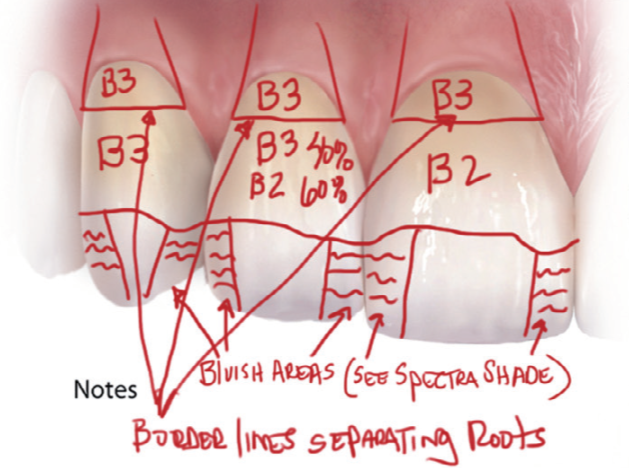
\includegraphics[width=0.5\textwidth]{grafiken/lab_card.png}
			\caption{Cutout of a lab card \citep{sharpling2014}}
	\label{fig:lab_card}
\end{figure}
\newline
The Figure \ref{fig:CrownProcesses} shows the sequential states of the dental crowns after each main process conducted by the dental technologist.First of all, the crowns have to be milled out of cylindrical blank which can provide enough bulk material for about 20 crowns. The milled crowns are colored via variety of brushes using  false colored inks to help the dental technician to visually differentiate the colored regions and the inks from each other, which do not possess their final color and have an extremely low contrast so that it is hard process for the human eye to recognize the borders of the different ink applied areas.


\begin{figure}[h]
	\centering
	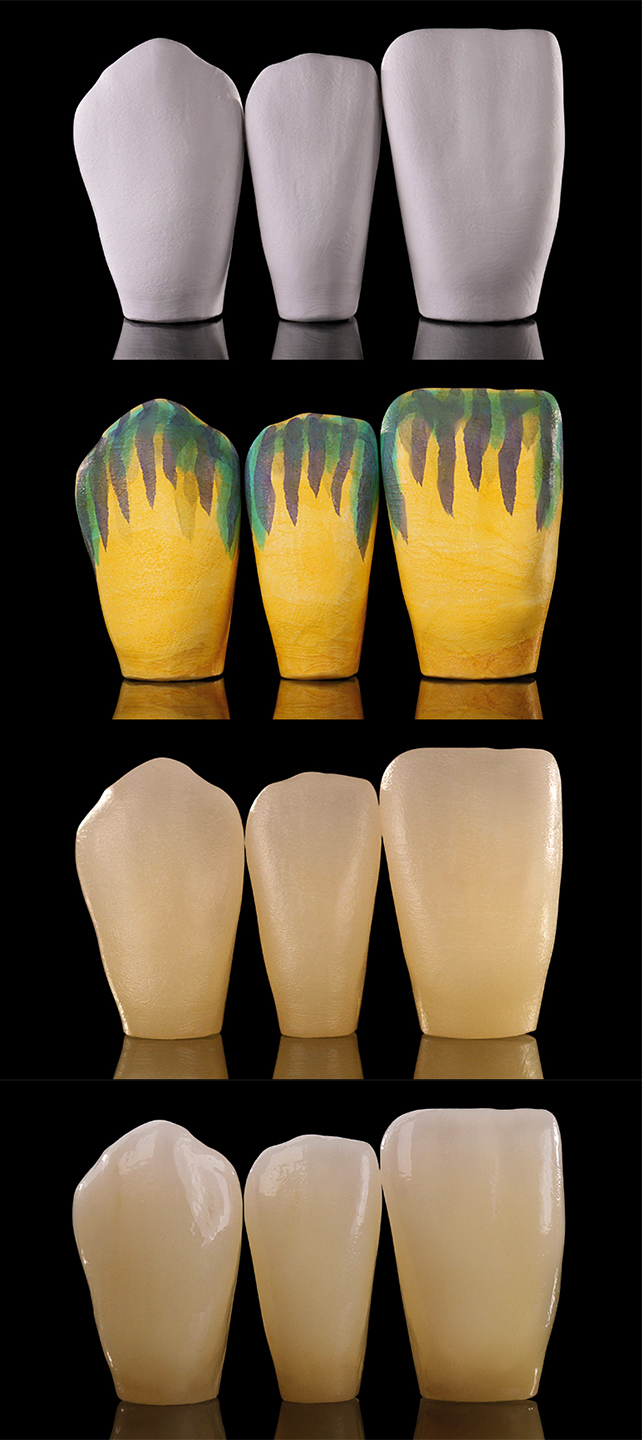
\includegraphics[height=0.6\textwidth]{grafiken/CrownProcesses.jpg}
	\caption{Making of dental implants \citep{zirkonzahn2018} }
	\label{fig:CrownProcesses}
\end{figure} 
 

Afterwards te colored dental crowns are sintered for the ceramic to reach its final strength. The false colors of the inks evaporate at temperatures above 1200\textdegree C and the metalionic ink becomes more visible providing the zirconia natural tooth like shade which roots from the depths of the ceramic structure. As a final process the crowns are masked and polished.



\chapter{Review of the State of the Research and Technology}
\label{sec:kritik_stand_technik}
The second stage which is the coloring process is the part this thesis is focused on. The coloring process is a qualitative procedure. The amount of ink to apply on the dents and edges of the crown are described in measures of brush strokes. The literature or the technical documentation does not provide a quantitative approach about the required amount of ink. In Figure \ref{fig:false_colored} one can observe how cumbersome it is to accomplish the full colorization of a crown. More importantly,if the batch size is large an important problem surfaces. The sequential teeth have to comply with the natural ones already present in the application area or the ones colored before. The shading tolerances cannot be allowed to be too high, because of the uncommon irregularity of the teeth colors this situation would cause for the patient. 
\newline
\begin{figure}[h]
	\centering
	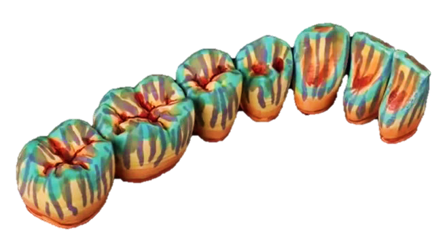
\includegraphics[width=0.6\textwidth]{grafiken/false_colored.png}
	\caption{False colored crowns after manual brushing \citep{zirkonzahn2018}}
	\label{fig:false_colored}
\end{figure}
\newline

There are already devices to check the generated shade as a quality control measure. The proactive measure to control the shade to be generated is premixing the coloring agent with the brightener at the factory to guarantee that the zirconia will have the predefined color after the sinter if the zirconia is soaked in to the ink or the ink is applied on the surface until saturation is reached.
For the printing process the amount of ink required for each shade, the time of depletion of the micro drops from the surface of the zirconia in the the porous structure and the size of the generated spot as well as the distribution of the ink depending on the radial distance from the center of the spot is of high interest.

\cleardoublepage
\counterwithout{figure}{section}
\counterwithout{table}{section} 
\counterwithout{equation}{section}
\counterwithin{figure}{chapter}
\counterwithin{table}{chapter} 
\counterwithin{equation}{chapter}


\chapter{Assignment}
\label{sec:aufgabenstellung}
 In frame of this thesis a process is to be developed for generation of the dental color shades using an inkjet printer.  The mechanic aspects of responsible for the movement are not included to the project. A stepper motor driven system responsible for the coordinated movement of the axes controlled by a SmoothieBoard v2-mini is provided by the project partner Bredent GmbH. The specifications of the printing system, like a single drop volume or the max printing distance and angle are to be determined. 
 
 Afterwards, an adequate droplet generator is to be selected. The diameter of the nozzle is as important as the driver technology generating the droplets, which has a direct effect on the optical resolution of the printed pattern. With piezoelectric droplet generators, smaller and faster drops are possible but electromagnetic ones are cheaper. The quantitative coloring behavior depending on the absorption characteristics of the dental ceramic is an unknown to the state of the research and the technology. The shades of the dental colors are to be brought about using the main colors with the highest saturation level and a brightener, which is a water based diluter with  an identical composition to the inks, except lacking the metal-ionic coloring agent. The proportions of the ink and the diluter is not the only parameter affecting the shade of the generated color, but also the application sequence can have a significant effect on the optical perception. Since the translucency of the dental zirconia effects the level of color reflection, the depth of the colored section can have an undeniable effect on the natural look of the dental crown. 
 
 At last, the generated shades are to be verified with the existing color standards. The receipt for each single shade generation has to be prepared. The deployed droplets are not expected to fly and settle on the contact point drying on the surface, but are expected to be absorbed and spread inside the porous material. This nature of the interaction between the ink in its fluid form and porous zirconia defines the system as a nonlinear three dimensional fluid dynamics problem. A model is to be generated taking the every compensational aspect of the nonlinear ink behavior, in order to achieve a point accurate color acquisition.
 
 

\chapter{Expected Advantages and Functions of the Solution}
One of the most important advantages is quantification of the coloring process followed by the printing process. Until this day, the crown coloring process is made by dental technologists all around the world. In other words, all of the dental replacements are partially handcrafted. In the market, hand crafted is another word for made by a craftsman, specifically for the unique owner of the product. Just as any other product on the market, the word handcrafted has a prominent effect on the price tag of the item. The word handcrafted also means the product has some tiny error, a nuance special for each unique sample. If the object of interest is a decor for the home of the consumer, it is one of the most welcome properties. However, if the object of interest is an implant, which is to be carried all the time on the comsumer's body as a part of the it, the property everyone is looking for is perfection. A perfect shape, color, consistency and harmony is a standard to evaluate the quality of the work done by the dentist and of course involving the dental technologist. The quantification of the coloring process is the most important advantage of the solution when it is considered looking from this aspect. Thus, the error can be terminated and the quality deviation can be limited to an acceptable variance. 

Another aspect to consider is the ink costs. Each of the ink bottles are labeled with the same price tag by the manufacturer. However, not all of the ink bottles contain a material worth the same value actually. The shades of the colors ranging from 1 to 3.5 are only diluted versions of the bottle with the shade 4.0. Buying the most concentrated tone and diluting it is here an economical solution, as it is in every other section of the industry. Also, the whole spectrum of shades can be obtained with only 4 ink bottles and a brightener by halftone printing. The required purchase variety, transportation costs, and the space requirement are all reduced with the usage of only the most saturated shades.

\chapter{Solution Structure}
The structural concept is based on the utilization of a 5-axis printing system. A basic microcontroller designed for the automation of the router systems is connected to stepper motors and encoders to control the coordinated printing processes. 4 base colors with the highest saturation levels (A, B, C and D4) are to be used with the brightener to color the dental zirconia, instead of 17 bottles consisting of 16 predefined shades plus the brightener. The amount of the brightener defines the shade of the color. Therefore, the space requirement of the machine is reduced. The inks and the brightener are continuously fed into a rotary distribution valve and are in their neutral status not flowing in any direction. As soon as the rotary valve opens the gate of any incoming pipe,the flow is permitted to the droplet ejector.  

\bigskip

\begin{figure}[H]
	\centering
	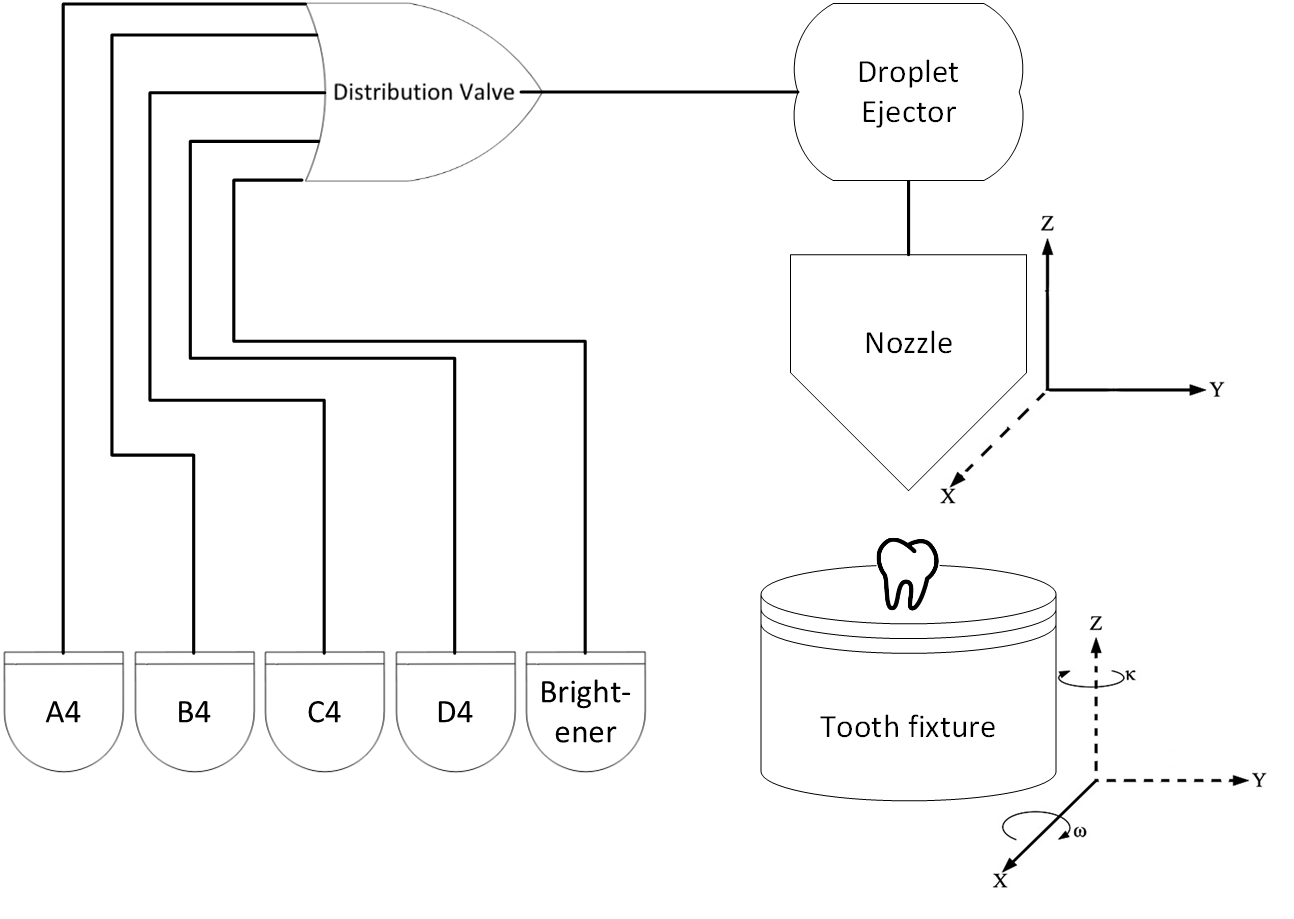
\includegraphics[width=0.9\textwidth]{grafiken/SolutionStructure.jpg}
	\caption{Solution Structure}
	\label{fig:SolutionStructure}
\end{figure} 

\bigskip

A serial communication between the controller and the rotary valve arranges the position of the rotary valve and the duration to hold on in that position. The required mixture is dosed and pulled by the droplet ejector and deployed through the nozzle, driven by the pressure difference between the ink bottles at the beginning of the cycle and the atmosphere. A 3-axis table and the 2-axis nozzle holder are responsible for the coordination of the flying drops and the point on the surface of the dental crown where the drops need to land during the printing process.

\chapter{Solution Processes}
\label{sec:Lösungsprozesse}
The process concept is realized in three stages. Each stage depends on the previous one and cannot be proceeded to, before the previous one is completed.

\bigskip

\begin{figure}[H]
	\centering
	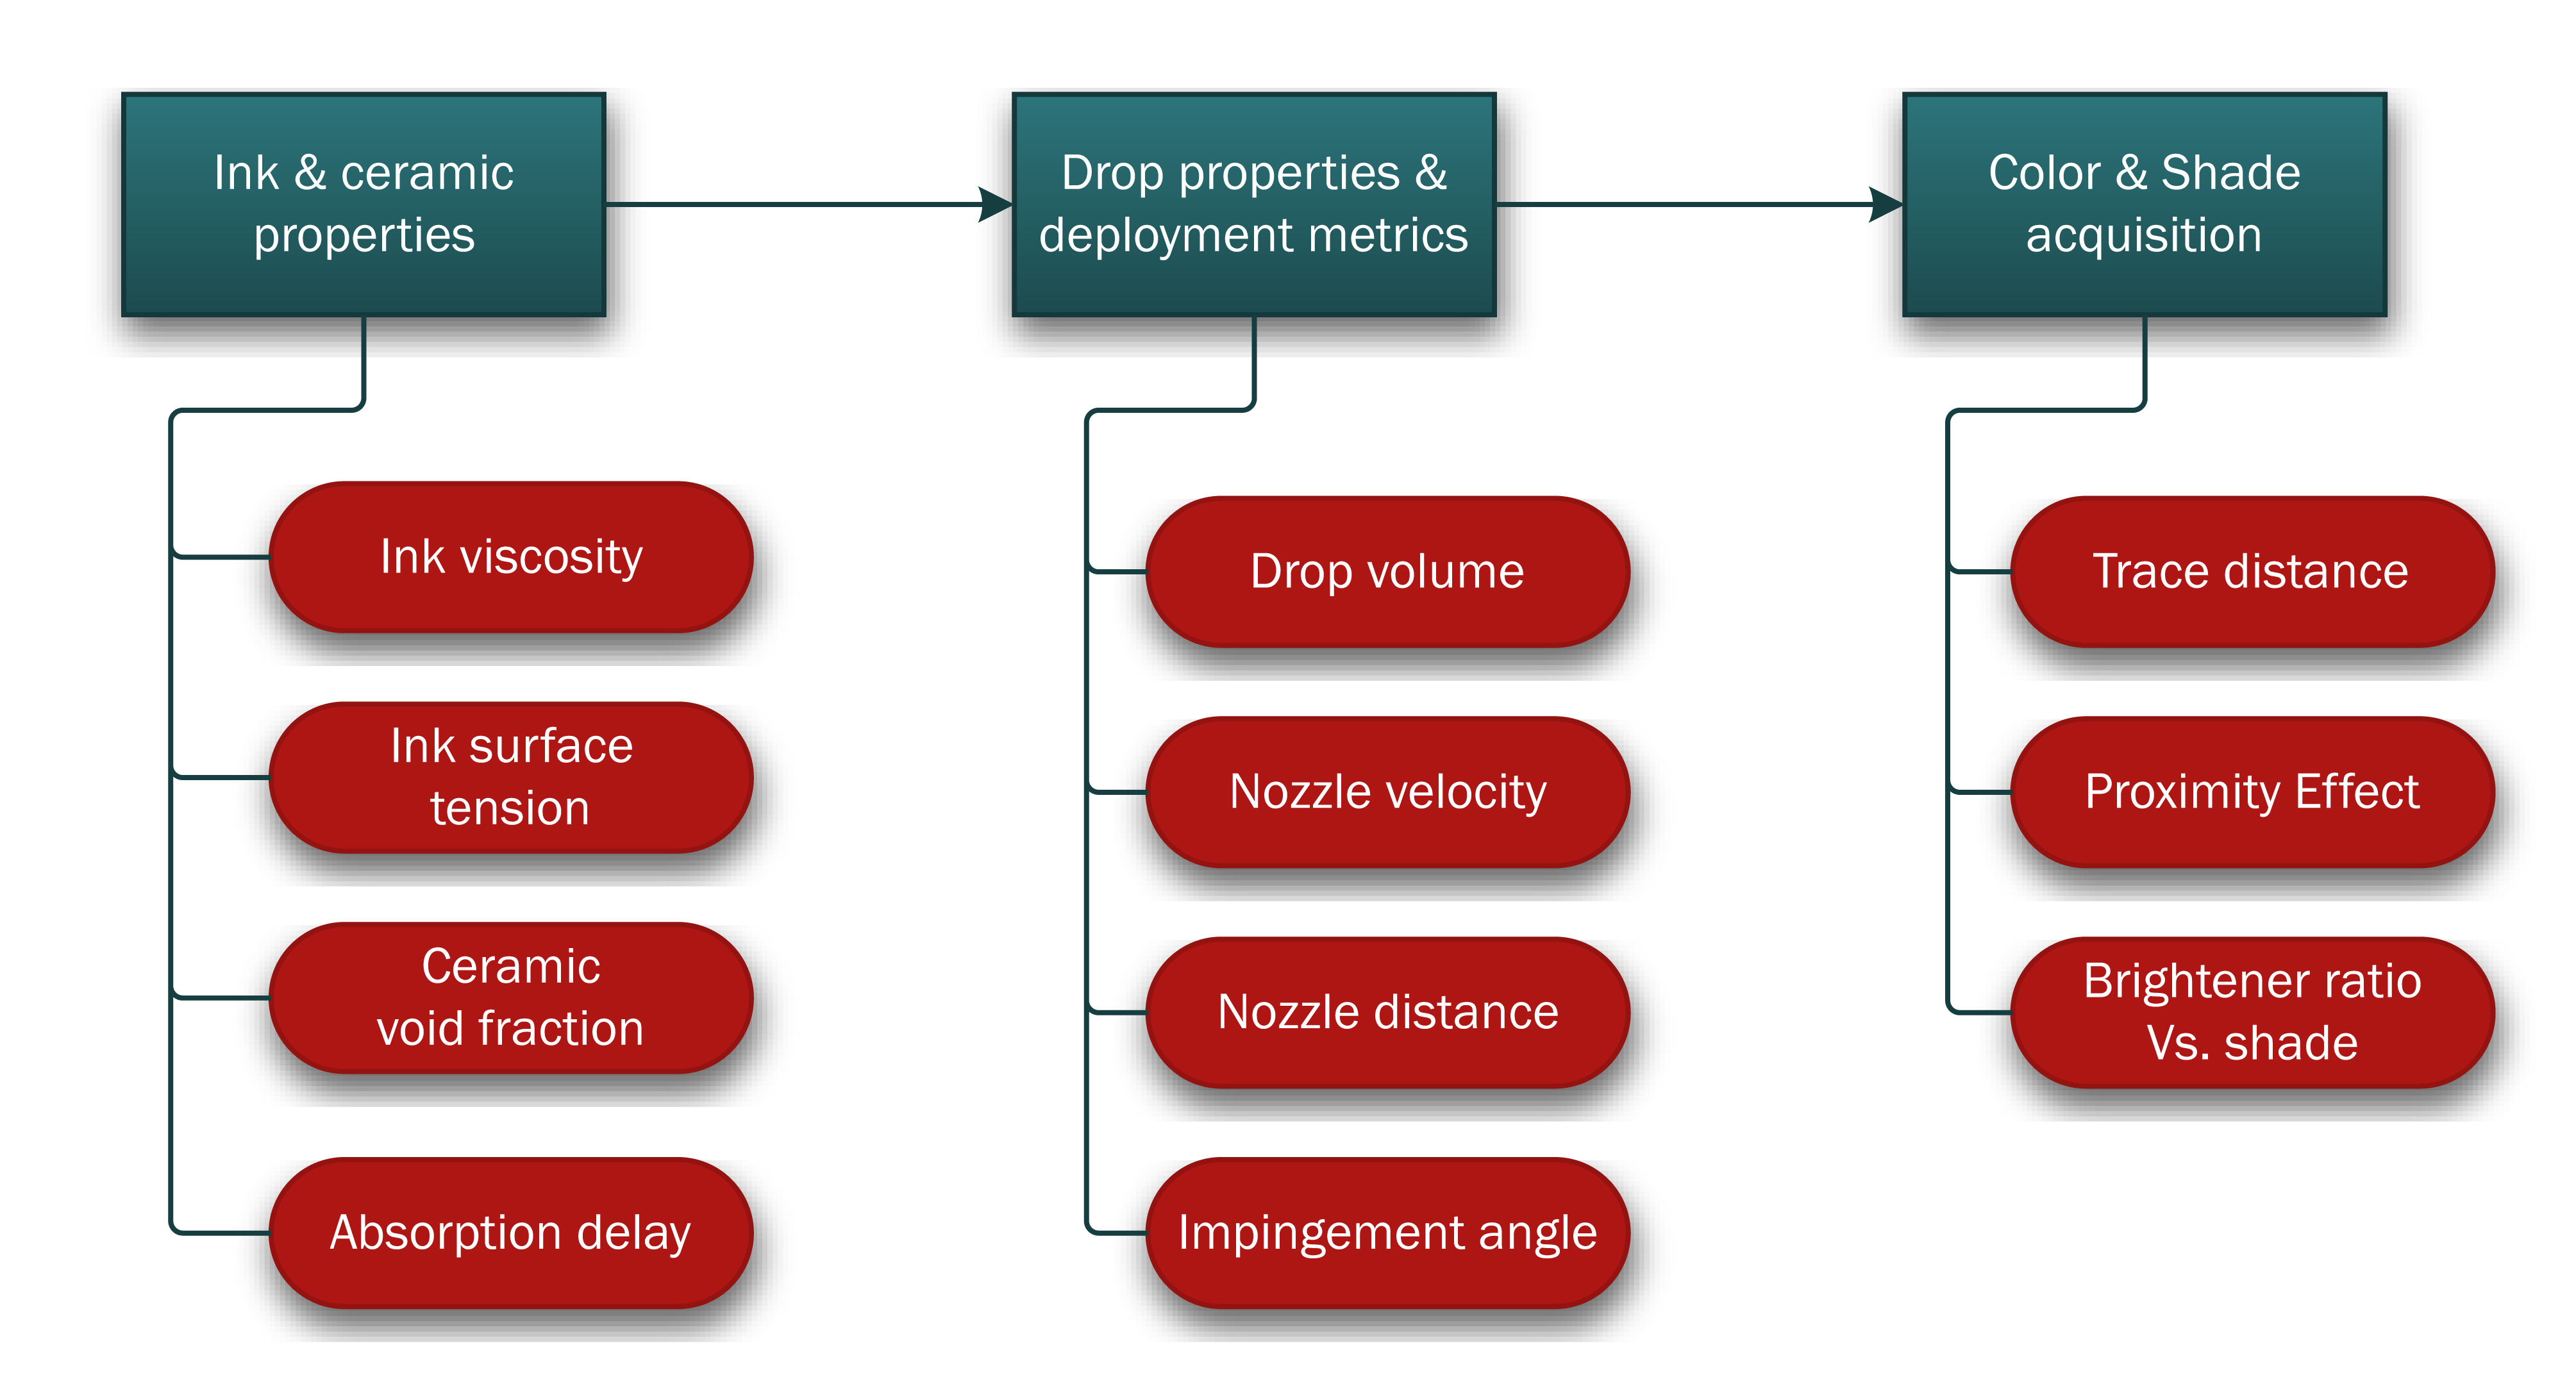
\includegraphics[width=0.9\textwidth]{grafiken/SolutionProcesses.jpg}
	\caption{Solution Processes}
	\label{fig:SolutionProcesses}
\end{figure} 

\bigskip


 First stage is finding the ink and ceramic properties, such as ink viscosity and surface tension, ceramic void fraction and ink absorption time. Depending on these experimentally acquired parameters the equations \ref{eq:InfTime} and \ref{eq:SpreadingDia} can be utilized  in the progress of the model generation for the drop deployment algorithm for an arbitrary pattern to be printed on the zirconia material. 
 
 Second stage is planned to help determine the parameters defining the printing system. It basically focuses on the settlement of drop properties and deployment metrics, which consist of drop volume, nozzle escape velocity of the drops, the optimal distance between the nozzle and zirconia surface and the angle between the drop projectile and the surface. The drop volume has to be determined as soon as possible, because it directly affects the selection of the actuator which is to be used as the drop ejector. Selection of a larger drop size means a shorter printing time. However it also means that the resolution is supposed to become lower. Due to the absorption characteristics of the zirconia material, a critical drop size is expected to cause a significant effect on the diameter of a painted spot. In other words, deploying the same amount of ink on the same spot using drops with a volume of smaller than 5 nL could give the same printed spot diameter.In comparison to the aforementioned drop volumes, using  10 or 20 nL drops to apply the same amount of ink on a single point could result with an unexpectedly larger spot size with lower central intensity. This critical drop size has to be determined, in order to proceed to the rest of the experiments.  
 
 The projectile velocity of the drops is one of the most important parameters affecting the printing system on a temporal basis and also the spreading characteristics of the ink within the porous medium. It is known that for Weber numbers higher than 50, the drops are expected to splash upon the impact with the surface \citep{clarke2002spreading}.
 
 \bigskip
 
 \begin{equation}\label{eq:weber}
 We=\frac{\rho rv^2}{\gamma}
 \end{equation}
 
 \bigskip
 
 The maximum distance of the nozzle to the zirconia surface has to be limited. The projectile of the droplets are not perfectly identical. There is a deviation of the impact point, because of the factors like a slight change of the nozzle escape angle of an arbitrary droplet or drag caused by the spontaneous fluctuation of the air flow inside the printing chamber. The longer the fly distance of the droplets are, the less accurately they will meet the same point. So the deployment distance for the droplets should be as short as possible. However on the other side the geometry of the crown creates the second boundary of the problematic. The concave structures on the upper side of the teeth carrying out the chewing function pose a collision danger with the nozzle. This is a situation where the printing angle is also influential. 
 
 The aspects to be considered under the third stage are employed to conduct an experimental approach to color and shade acquisition. In order to arrive there some parameters have to be determined. Firstly the appropriate trace distance for the selected drop size is to be concluded, depending on the experiment with varying trace distances, which is the distance between two sequential lines on the printed surface. The proximity effect is the second nonlinear parameter affecting the print resolution and color distribution, which refers to how the proximity of two colored areas affect the shade of the uncolored area in between.Finally the dependency of the shade on the brightener ratio is to be determined. For a liquid inside a bottle it is very easy to come to a final conclusion. However, the porous translucent medium has a huge influence on the perceived shade, because of the  reflections form various depths of the material and photons following diverse paths through the sintered zirconia to the eye of the observer.
 
 All of the aforementioned tasks are to be carried out so at the end a model can be generated. This model has to work as an algorithm to calculate the input pattern for a desired arbitrary shade map of a dental crown geometry. The coloring behavior on the printed sample has to be compared with the virtually printed geometrical model.
 

\chapter{Distinctive Features of the Solution}
\label{sec:Unterscheidungsmerkmale}
The most contemporary dental laboratory of today still has to do the coloring process manually. A dental technologist uses brushes to apply tens of bottles of ink shades to the dental crowns one by one following the procedures described by dental zirconia ink manufacturers. Coloring each tooth takes about 5 minutes and about 100 precise brush strokes. This is a process which requires a high patience and repeatability. This project is the first automated printing approach in dental coloring sector. With the automation of the procedure many advantages are expected. The accuracy of shade acquisition is to be guaranteed because of the quantified and digitalized coloring procedure. The variation between the sequential teeth are to be minimized. Shorter lead times can be realized upon the optimization of the printing method, which is to be accompanied by lower costs due to the automation and shortened process time.

Another novelty of the project is the discontinuation of the requirement for a bottle for every single shade of each color. The lighter shade of each color are only bottle mixtures of the brightening fluid and the darkest shade of that color by the manufacturer. The mixtures do not posses a linear ratio for the contained ink and brightener depending on the color shade. The mixture is prepared considering the end shade to be acquired on the zirconia. This project makes it possible for the first time to generate the shades using the darkest base colors and a brightener, thanks to the digitalization of the coloring procedure.

\chapter{Experiments}

Before moving on to the experiments I want to show you the 5 axis printing system prototype provided by Bredent GmbH. for conduction of the experiments. 
It utilizes a single nozzle print head with a piezoelectric valve to generate the droplets. Ink selection, positioning and drop generation commands are given with a G-Code.

\bigskip

\begin{figure}[H]
	\centering
	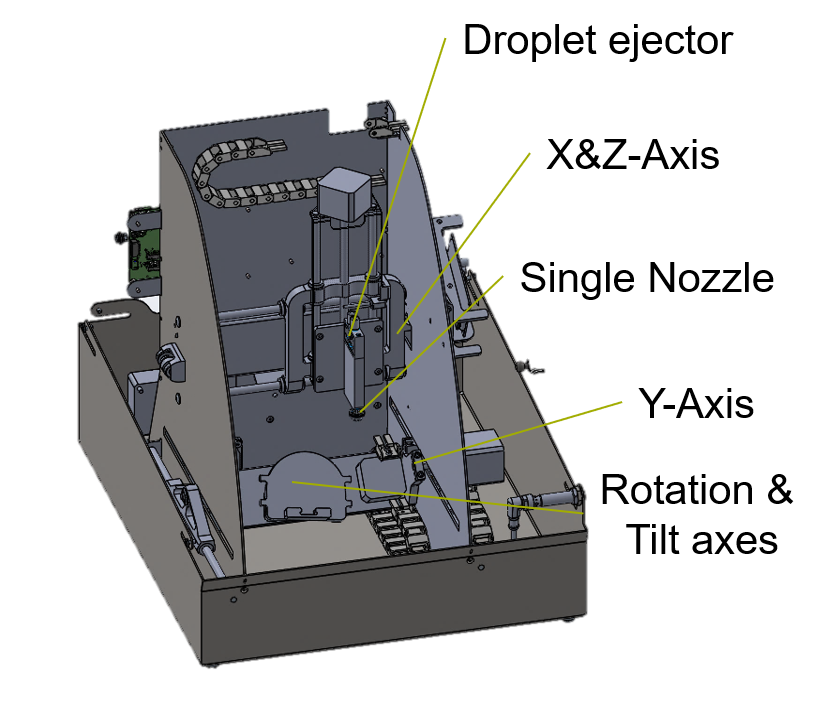
\includegraphics[width=0.7\textwidth]{grafiken/PrototypeText.png}
	\caption{5 axis printer design for dental ink (Matthias Leininger, Bredent GmbH)}
	\label{fig:Prototype}
\end{figure} 

\bigskip

\section{Material Properties}
For a dental technician it is completely trivial how viscous the ink is but for an automated printing  process the quantization of the properties is highly important. In the first experiment, the properties of the coloring agents A1, A2 and A3.5 are determined and compared to those of water. The inks have a similar density to water, but with increasing coloring agent the surface tension gets lower and the viscosity gets 3 times higher when compared to water. Also, a porosity measurement for the zirconia is conducted, which revealed a 43 percent void fraction. The raw volumetric porosity measurements are 43.09,	43.00 and 43.70. The consistency of the results is also a sign for randomly close packed zirconia powder during the manufacturing procedure. Otherwise the irregular packing would inhibit the fluid drainage and cause macro voids inside the porous material after the dissipation of the impregnating liquid, which would also lead to porosity measurements with a significantly large standard deviation. 

\bigskip

\begin{figure}[H]
	\centering
	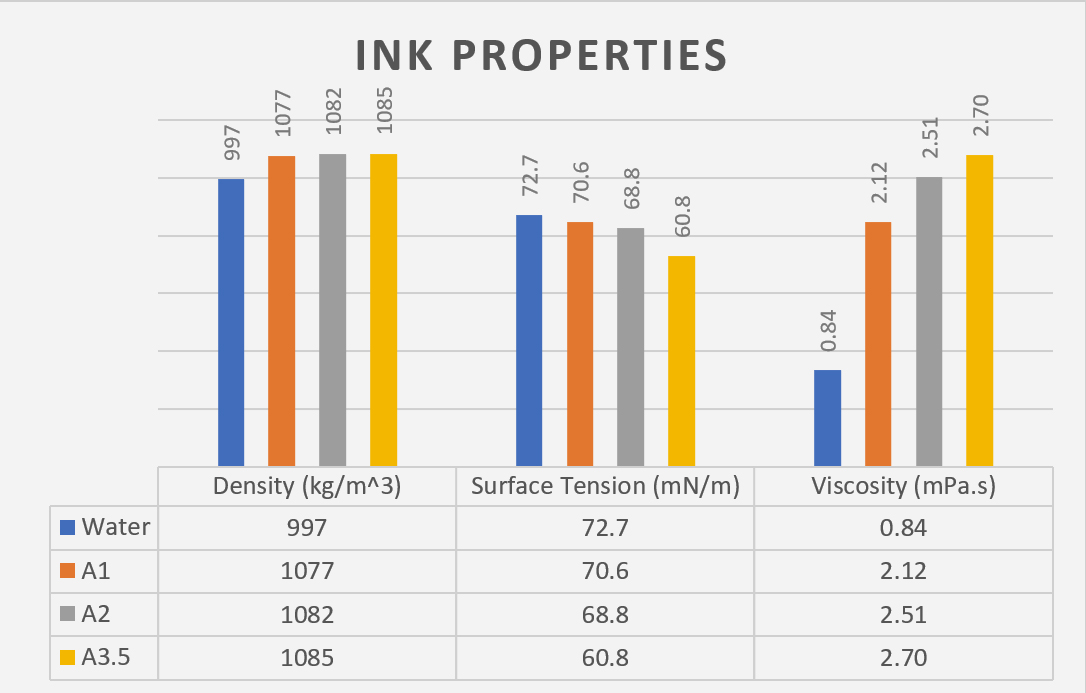
\includegraphics[width=0.8\textwidth]{grafiken/InkProps.jpg}
	\caption{Ink Properties}
	\label{fig:InkProps}
\end{figure} 

\bigskip

The most important outcome of this experiment is high values of viscosity observed for the inks, in comparison to water. This situation provides numerous advantages for the drop generation part of the process. The higher viscosity of the ink helps reduce the occurrence of the satellite drops.

\section{Ink Concentration vs. shade without Lateral Flow}

The dental colors appearing after the sintering process have to be assigned to specific ink concentrations. When a pattern is printed on the zirconia surface a part of the ink deployed on the target area escapes the region where t is supposed to be through lateral diffusion in the pores of the material. That is the reason one observes a spread distribution of color intensity. This can be inhibited if the whole material is printed with the same amount of ink to assure a homogeneous color intensity throughout the whole surface to obtain the theoretically achievable shades without the influence of lateral diffusions inside the material.

In order to conduct the experiment, 10 zirconia plates are prepared in a square form. The surface of the plates are imprinted with the amount of ink which is equal to the 0\%, 10\%, 20\%, 30\%, 40\%, 50\%, 60\%, 70\%, 80\%, 90\% und 100\% of the calculated porosity of the zirconia plates. The color intensities are calculated later with the results of the PSF experiment.




\section{Absorption Time}
The second experiment is about the absorption time of the droplets which limits the printing time. Before the first drop is absorbed, a second drop should not land on the same spot. This would lead to accumulation of the liquid on the surface and eventually they would flow in the direction of the first drop because of the surface which is already wetted. The target accuracy of the drop deployment system would lose all of its importance. The resolution would be also sacrificed alongside the target accuracy, due to the accumulated liquid on the surface. The absorption time is formulated by Markicevic et al. as in equation \ref{eq:InfTime}.

Depending on the Eötvös rule, the surface tension of any Newtonian liquid declines with climbing temperature values. For water the formula is generated as:

\bigskip

\begin{equation}\label{eq:watergamma}
\gamma =0.07275 \cdotp(1-0.002\cdotp(T-291))
\end{equation}

\bigskip

Arrhenius-Andrade-Relation defines the viscosity of any Newtonian fluid depending on the temperature in the equation \ref{eq:viscosity}.  

\bigskip

\begin{equation}\label{eq:viscosity}
\eta =\eta_0 \cdotp exp(\frac{E_A}{R\cdotp T})
\end{equation}

\bigskip

The exponential reduction of the viscosity  versus the proportional decrease of the surface tension would be expected to result with a cumulative decrease of the absorption time with climbing temperatures.

Single drops with a volume of 100 nL are deployed on the sawn and milled surfaces. The time between the landing and complete absorption was measured 4 times for each surface structure at the temperatures 20\textdegree C, 30\textdegree C, 40\textdegree C, 60\textdegree C and 80\textdegree C.

\bigskip

\begin{figure}[H]
	\centering
	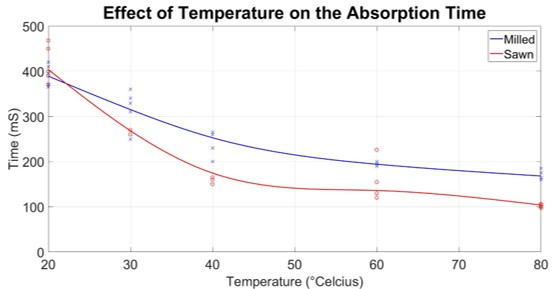
\includegraphics[width=0.8\textwidth]{grafiken/AbsorptionTime.jpg}
	\caption{Effect of heat on the absorption time}
	\label{fig:AbsorptionTime}
\end{figure} 

\bigskip

Analyzing the collected measurements, it can be concluded that a 60\textdegree C increase of the zirconia plate leads to about 50\% reduction of the absorption time. These values are to be employed for a curve fitting to be implemented to the shade model at the final stage of the thesis.
 
\section{Drop Size Selection}
The purpose of the third experiment is deciding for an adequate drop size.A larger drop size results in shorter print duration. However they also tend to expand the spot area more compared to the smaller drops,even though the porous material is not close to being saturated, which is a serious problem for the resolution. Depending on the drop size the drop generation method is to be selected. 
\bigskip
\begin{figure}[H]
	\centering
	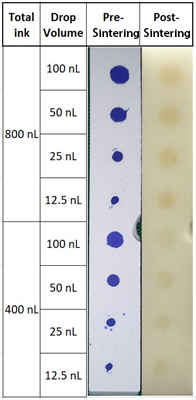
\includegraphics[width=0.36\textwidth]{grafiken/DropSize.jpg}
	\caption{Effect of the drop size on the spot area}
	\label{fig:DropSize}
\end{figure} 
\bigskip
In the figure \ref{fig:DropSize} one can see a printed zirconia specimen. Each spot on the upper half has a total ink volume of 800 nL and the ones on the bottom half 400 nL. These spots are printed using drops with volumes of 100, 50, 25 and 12.5 nL.The first image shows the spots right after printing. The second one shows the surface after furnacing.

\bigskip

\begin{figure}[H]
	\centering
	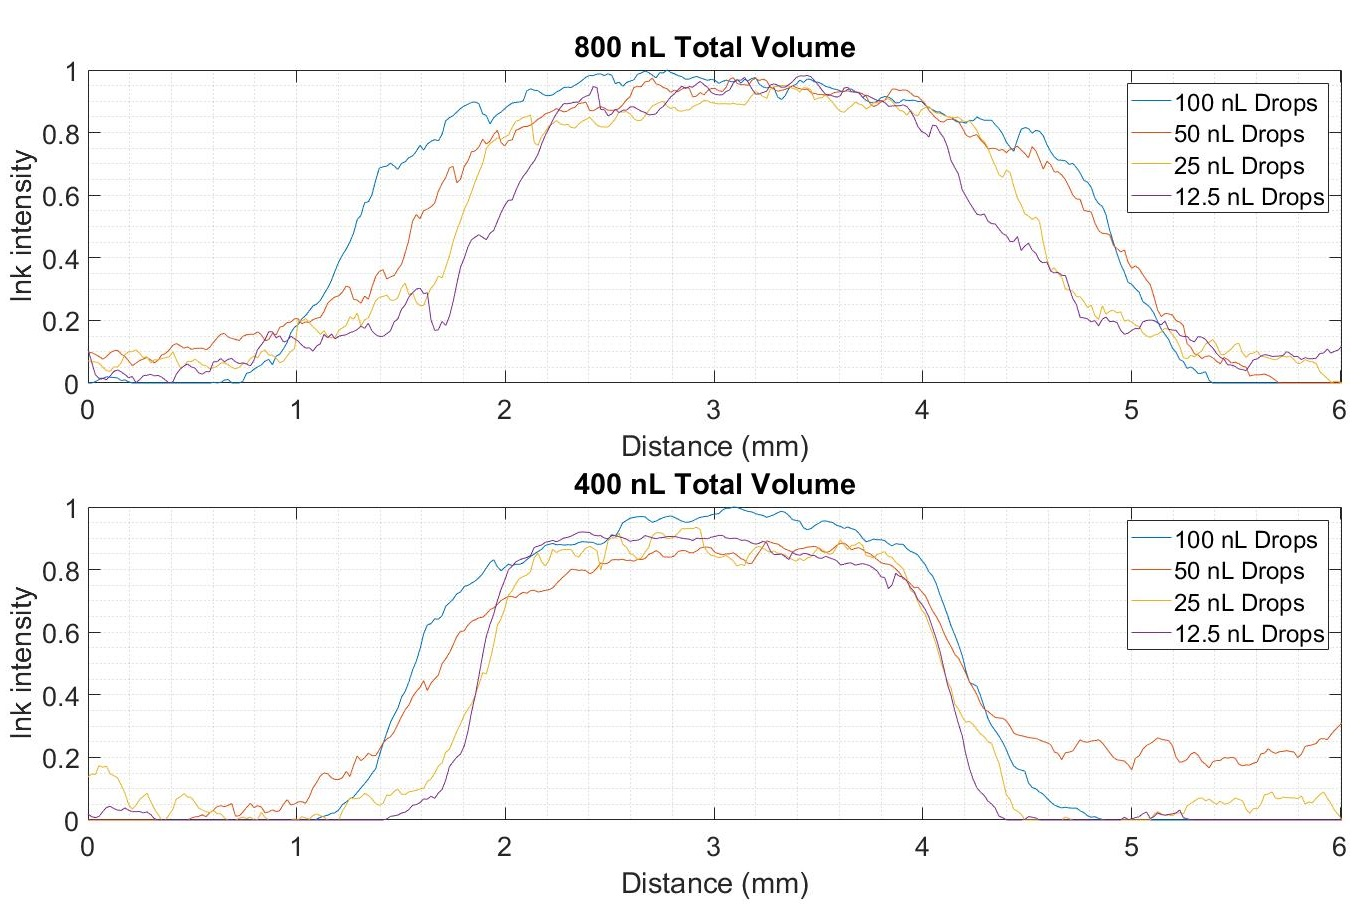
\includegraphics[width=1\textwidth]{grafiken/SpotArea.jpg}
	\caption{Comparison of the spot area results depending on the drop size}
	\label{fig:SpotArea}
\end{figure} 

\bigskip

The graphs show the ink intensity along the red lines and the spreading of the ink in lateral direction for each drop volume. 12.5 and 25 nL drops result in a similar spot diameter but the spots tend to get significantly larger with 50 and 100 nL Drops.

\section{Proximity}
The proximity effect describes in the case of dental printing the coloring of the unprinted area between two printed areas proximate to each other. The closer the printed areas are, the saturated does the unprinted area in between become.

If the color change of the unprinted area can be described depending on the ink concentration and distance between the printed areas, the effect of the proximity can be implemented to the model.
\bigskip

\begin{figure}[H]
	\centering
	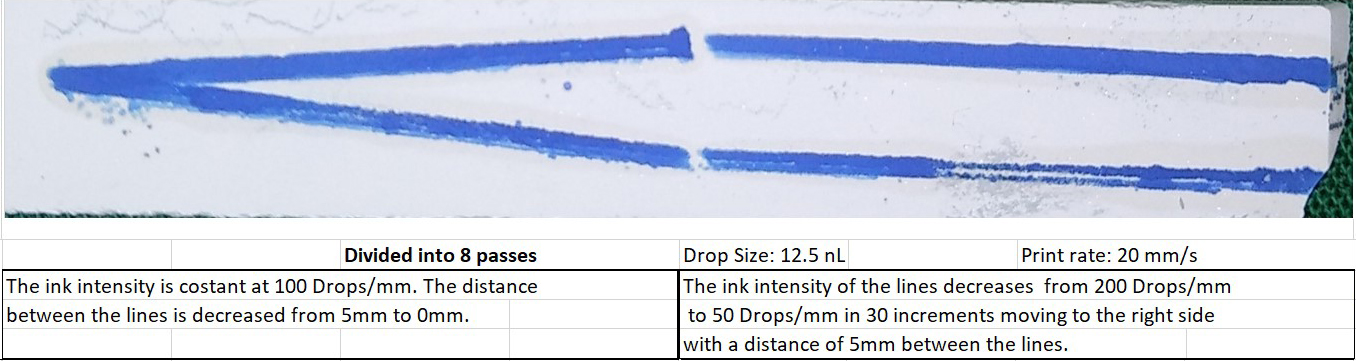
\includegraphics[width=1\textwidth]{grafiken/proximityprint.jpg}
	\caption{Comparison of the spot area results depending on the drop size}
	\label{fig:proximityprint}
\end{figure} 

\bigskip

A pattern with varying droplet concentration and another pattern with varying distance between two lines was printed on the zirconia.

\bigskip

\begin{figure}[H]
	\centering
	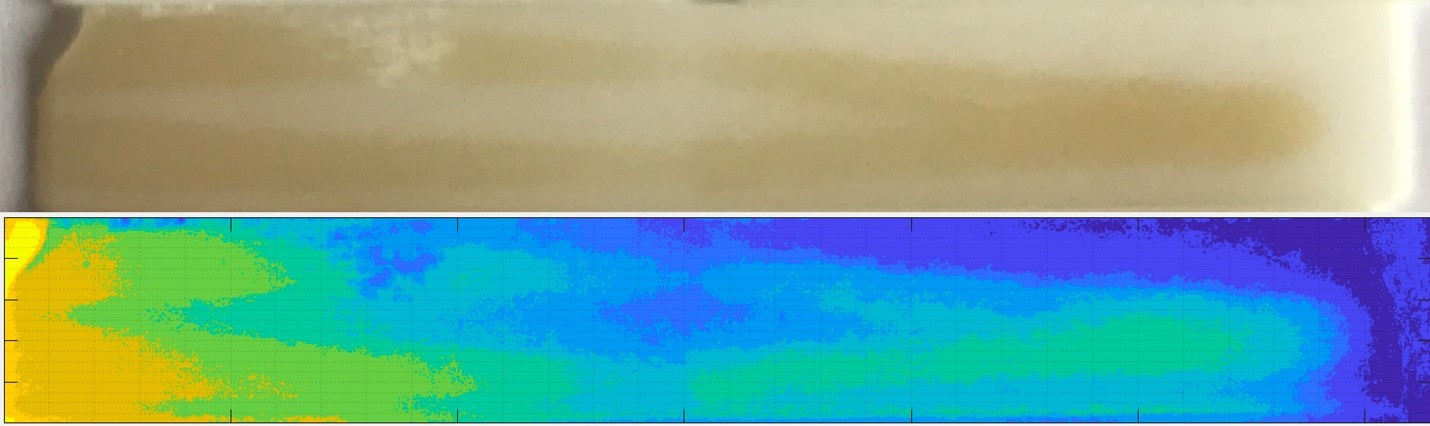
\includegraphics[width=1\textwidth]{grafiken/proximitysinter.jpg}
	\caption{Comparison of the spot area results depending on the drop size}
	\label{fig:proximitysinter}
\end{figure} 

\bigskip

Observing the Figure \ref{fig:proximitysinter}, one can qualitatively conclude, that the proximity has a significant effect on the coloring behavior.


\section{Printing angle}
The dental crowns do not always present convex features. The chewing surface can rarely possess even some under cut geometries. In such cases it is not possible for a droplet to land on the zirconia surface vertically and for some known areas, the printing process has to be conducted on skew surfaces. 

If the lateral momentum of the droplet are high enough at moment of the impact on the surface, the printed pattern can look like it has a motion blur effect. It is also possible that the resolution gets lower because of the lateral flow of the drops on the surface. There has to be some critical angle, at which such disadvantages become inevitably  significant. The maximum milling angle used for the dental crowns is declared by Bredent GmbH to be 30\textdegree. So, an experiment to test the effects of printing on a skew surface up to an angle of 45\textdegree is supposed to be comprehensive enough.

	\bigskip

	\begin{figure}[H]
		\centering
		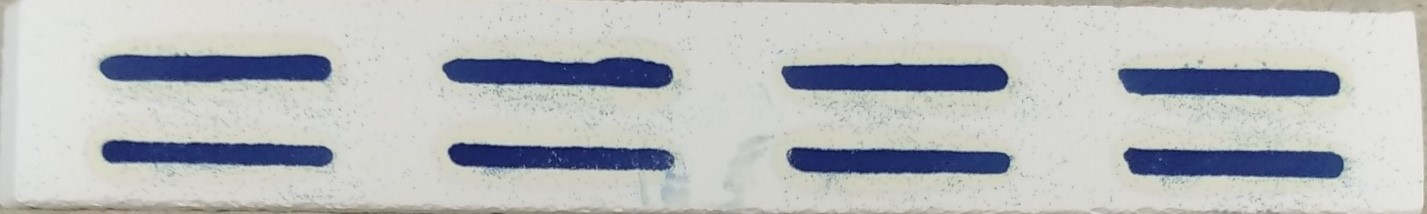
\includegraphics[width=1\textwidth]{grafiken/angleprint.jpg}
		\caption{Comparison of the spot area results depending on the drop size}
		\label{fig:angleprint}
	\end{figure} 

	\bigskip

In order to test the effect of printing on a skew surface to parallel lines are printed on the surface which have a distance of 4mm 4 times, while the zirconia specimen was standing at angles 0\textdegree, 15\textdegree, 30\textdegree and 45\textdegree. The printed sample can be seen in the figure \ref{fig:angleprint}
The lines were generated using 25 nL droplets with a drop density of 50 drops per mm.

\section{Point Spread Function}


The halftone tonality is greatly affected by optical dot gain, a phenomena caused by the photon diffusion inside the medium. The point spread function (PSF) is one of the ways to model the optical dot gain. The derivation of an appropriate PSF is accomplished through solving the radiative transfer equation, which leads to a PSF in terms of the scattering and absorption coefficients of the medium. This PSF is then used for calculating the average diffusion distance of the photons inside medium. It is shown in the work of Rogers that the Z-sum, which can be expressed explicitly, can be estimated by $\mu^{-s}$, where $\mu$ is the fractional ink coverage and s has values between 0 and 1.  The interrelationship  between the PSF  approach and the probability approach is proven to be strong. \citep{rogers2015point}

In words of a less complexity, the generated drops do not act as if they have definitive borders. In the contrary, the ink concentration decreases in the distal direction in a point symmetrical Gaussian distribution form. Because of that one can not simply measure the diameter of a drop with direct comparison methods. Point Spread Function is used to define the distribution of the observed color depending on the distribution of the ink taking also the optical dot gain in consideration.

The drops are expected to have a high color intensity in the middle That middle point is going to be the center of the Gaussian distribution.The points with an equal distance from the middle are supposed to present a point symmetrically identical color intensity.

\bigskip

\begin{figure}[H]
	\centering
	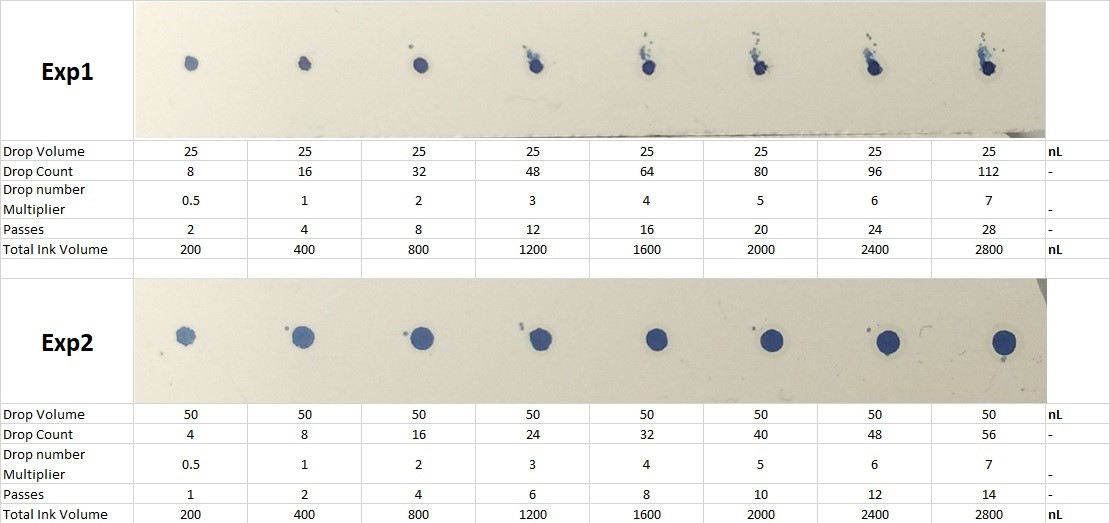
\includegraphics[width=1\textwidth]{grafiken/psfprint.jpg}
	\caption{Comparison of the spot area results depending on the drop size}
	\label{fig:psfprint}
\end{figure} 

\bigskip

In order to inspect the Gaussian distributions of ink in cases of different total ink amounts and different drop sizes 8 spots are printed using drops with volumes of 25 nL and 50 nL. The total ink volumes for the spots on each plate are identical and equal to 200 nL, 400nL, 800nL, 1200 nL, 1600 nL, 2000 nL, 2400 nL and 2800 nL.

The results of this experiment are necessary for the reverse calculation of the required ink amount. Depending on the calculations a map can be generated for the amount of drops and target positions to deploy these drop, in order to acquire a desired shade distribution as an outcome.   

\cleardoublepage
\counterwithout{figure}{section}
\counterwithout{table}{section} 
\counterwithout{equation}{section}
\counterwithin{figure}{chapter}
\counterwithin{table}{chapter} 
\counterwithin{equation}{chapter}


\chapter{Summary and Outlook}
The coloring process of the dental crowns based on the Zirconia ceramics is a necessity because of the plain white appearance of the material with a 49\% translucency. The coloring process is realized through utilization of the metal-ionic inks. The sintering procedure binds the ceramic powder to provide a dental material with a high structural strength and also generates the color via oxidizing the metal-ionic at temperatures about 1200\textdegree C. Depending on the type of the ink classified by the groups of A, B, C and D, the color is defined and the concentration of the applied color determines the shade of the application area. Since the coloring process of the dental zirconia is not a two dimensional paint application process, but a 3 dimensional ink distribution problematic, due to the depth dependent luminescence of the dental problems, the digitalization of the procedure is not as simple as it is for a desktop printer. 

If the subject is approached from the perspective of the current state of the technology and research, it can be said that the coloring process is a complete manual procedure. The ink is applied on the surface by the dental technologist via a brush. The printing of the zirconia with a dental ink utilizing microdrops is an uncharted area, but there is a good amount of research conducted in the fields of microdrop generation and absorption behavior of porous materials. Conclusive experiments are done by Starov at el. to formulate the absorption time and spreading distance of a deployed single ink drop, which have constructed the backbone of the mathematical aspect of this thesis.

Utilizing a 5 axis router, the drop deployment procedure is automated. As color reservoirs 4 ink bottles with the highest saturation levels of the colors A, B, C and D are used with a brightener to achieve the shades of each color. The system is utilized to conduct some experiments to develop a model for the printing process. Ink and ceramic properties like the ink viscosities and surface tensions are obtained, as well as the ceramic porosity. The inks have a higher viscosity than water, which helps to extinguish the satellite drops. The porosity of the zirconia is obtained to be 43\%, which defines the volume to be filled with the ink and the brightener.

In summary, the printing speed can be accelerated with shorter absorption durations which are proved to decline 50\% with a 60\textdegree C increase of the temperature. The other most most important factor affecting the printing speed is the volume of a single drop. The most optimum drop volume is found out to be 25nL when the printing resolution is consider as the key factor. Printing experiments up to a distance of 20mm cause no significant quality variance. The printing measurement were replied at angles of 0\textdegree \space, 15\textdegree \space, 30\textdegree \space and 45\textdegree \space and result was the same. Printing quality was as good as 0\textdegree \space  when the process was replied at 45\textdegree \space .The effect of proximity plays a significant role in the printing trace distance. For the ink intensity of 1250 nl/mm, which is approximately the fully saturated ink amount for the trace on the test sample, the optimum trace distance  was observed to be 3mm. Afterwards the shade generation method is inspected in a discontinuous method rather than continuous lines to eliminate the effect of the neighboring regions with high ink amounts. For the 25 nl and 50 nl drop volumes a total ink amount of 2000 nl can be said to reach the aimed color intensity with inevitable lateral ink spreading. Charting of the color shade vs the ink amount is not an efficient approach to the shade generation process because of the different spreading ranges caused by different liquid amounts. The point oriented shade acquisition approach can be realized with interlayered deployment of brightener and ink until reaching the total liquid volume of 2000 nl. The brightener to ink ratios for target shade acquisition are yet to be analyzed in order to generate a model for the automated printing process. In the last experiment it was observed that smaller FWHM could only be observed with lower ink amount. It could be considered to generate inks for the printing purposes with higher saturation levels, in comparison to the inks on the market, especially for the printing process. Finally a model can be generated utilizing the point spread function analysis and optical dot gain phenomenon in association, in order to predestine the perceived color at the end of the sintering process. 

%Verhindern von Seitenumbrüchen innerhalb eines Eintrages im Literaturverzeichnis
%\setlength{\bibsep}{2ex plus2ex minus.5ex}

\cleardoublepage
%\bibliographystyle{masterarbeit
\bibliographystyle{eigenerBibStyleEN}
\bibliography{literatur}

\cleardoublepage
\listoffigures

%\include{Anhaenge}

\end{document}

